
\documentclass[nooutcomes]{ximera}
%\documentclass[space,handout,nooutcomes]{ximera}

% For preamble materials

\usepackage{pgf,tikz}
\usepackage{mathrsfs}
\usetikzlibrary{arrows}
\usepackage{framed}
\usepackage{amsmath}
%\pgfplotsset{compat=1.16}

\graphicspath{
  {./}
  {algorithms/}
  {../algorithms/}
}

\pdfOnly{\renewenvironment{image}[1][]{\begin{center}}{\end{center}}}

%%% This set of code is all of our user defined commands
\newcommand{\bysame}{\mbox{\rule{3em}{.4pt}}\,}
\newcommand{\N}{\mathbb N}
\newcommand{\C}{\mathbb C}
\newcommand{\W}{\mathbb W}
\newcommand{\Z}{\mathbb Z}
\newcommand{\Q}{\mathbb Q}
\newcommand{\R}{\mathbb R}
\newcommand{\A}{\mathbb A}
\newcommand{\D}{\mathcal D}
\newcommand{\F}{\mathcal F}
\newcommand{\ph}{\varphi}
\newcommand{\ep}{\varepsilon}
\newcommand{\aph}{\alpha}
\newcommand{\QM}{\begin{center}{\huge\textbf{?}}\end{center}}

\renewcommand{\le}{\leqslant}
\renewcommand{\ge}{\geqslant}
\renewcommand{\a}{\wedge}
\renewcommand{\v}{\vee}
\renewcommand{\l}{\ell}
\newcommand{\mat}{\mathsf}
\renewcommand{\vec}{\mathbf}
\renewcommand{\subset}{\subseteq}
\renewcommand{\supset}{\supseteq}
\renewcommand{\emptyset}{\varnothing}
\newcommand{\xto}{\xrightarrow}
\renewcommand{\qedsymbol}{$\blacksquare$}
\newcommand{\bibname}{References and Further Reading}
\renewcommand{\bar}{\protect\overline}
\renewcommand{\hat}{\protect\widehat}
\renewcommand{\tilde}{\widetilde}
\newcommand{\tri}{\triangle}
\newcommand{\minipad}{\vspace{1ex}}
\newcommand{\leftexp}[2]{{\vphantom{#2}}^{#1}{#2}}

%% More user defined commands
\renewcommand{\epsilon}{\varepsilon}
\renewcommand{\theta}{\vartheta} %% only for kmath
\renewcommand{\l}{\ell}
\renewcommand{\d}{\, d}
\newcommand{\ddx}{\frac{d}{dx}}
\newcommand{\dydx}{\frac{dy}{dx}}


\usepackage{bigstrut}


\newenvironment{sectionOutcomes}{}{}

\usepackage{array}
%\setlength{\extrarowheight}{-.2cm}   % Commented out by Findell to fix table headings.  Was this for typesetting division?  
\newdimen\digitwidth
\settowidth\digitwidth{9}
\def~{\hspace{\digitwidth}}
\def\divrule#1#2{
\noalign{\moveright#1\digitwidth
\vbox{\hrule width#2\digitwidth}}}


\title{Decimal Representations}
\author{Bart Snapp and Brad Findell}
\begin{document}
\begin{abstract}
Problems about Decimals.
\end{abstract}
\maketitle


%\begin{problem}
%Problem
%\begin{freeResponse}
%\begin{hint}
%Hint
%\end{hint}
%\end{freeResponse}
%\end{problem} 


\subsection*{Exercises}

\begin{problem}
What does $3.417$ mean in the base-ten place-value system?  Using the rectangle below as $1$, draw a picture the illustrates the place-value meaning of $3.417$.  Draw as accurately as you can, indicating how the picture would be drawn perfectly (if you could).  Indicate whether your model is primarily about length, area, or something else.  

\vspace{.5cm}
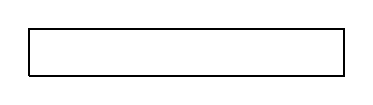
\begin{tikzpicture}
\draw [thick] (0,0) -- (4,0) -- (4,.6) -- (0,.6) -- (0,0);
\end{tikzpicture}
\end{problem}

\begin{problem}
Plot $3.417$ on each of the following number lines, zooming in to show how to make the placement more accurate at each step.  Draw dotted curves (as shown) to indicate where the zooming takes place, and label the large tick marks on each number line.  
\vspace{0.5cm}

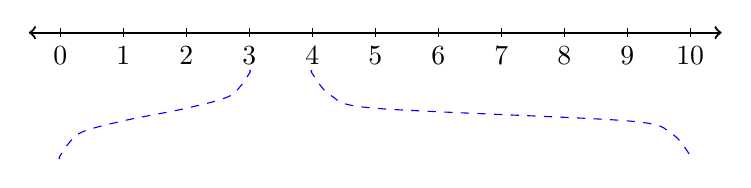
\begin{tikzpicture}[scale=0.8]
% a straight line segment
\draw [thick, <->] (-0.5,0) -- (10.5,0);
% the ticks and their labels
\foreach \x  in {0,...,10}
  \draw[xshift=\x cm] (0pt,2pt) -- (0pt,-2pt) node[below,fill=white] {\the\numexpr\x \relax};

\draw[dashed, blue] plot [smooth] coordinates{(3,-0.6) (3,-0.65) (2.7,-1) (2,-1.2) (1,-1.4)  (0.3,-1.6) (0,-1.95) (0,-2)};
\draw[dashed, blue] plot [smooth] coordinates{(4,-0.6) (4,-0.65) (4.3,-1) (5,-1.2) (9,-1.4)  (9.7,-1.6) (10,-1.95) (10,-2)};
\end{tikzpicture}

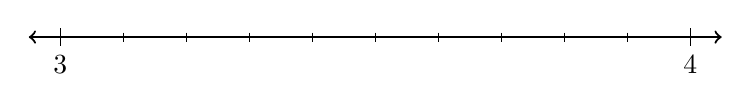
\begin{tikzpicture}[scale=0.8]
% a straight line segment
\draw [thick, <->] (-0.5,0) -- (10.5,0);
% the ticks and their labels
 \draw[xshift=0 cm] (0pt,4pt) -- (0pt,-4pt) node[below,fill=white] {\the\numexpr3 \relax};
\foreach \x  in {1,...,9}
  \draw[xshift=\x cm] (0pt,2pt) -- (0pt,-2pt);
 \draw[xshift=10 cm] (0pt,4pt) -- (0pt,-4pt) node[below,fill=white] {\the\numexpr4 \relax};
\end{tikzpicture}

\vspace{0.8cm}

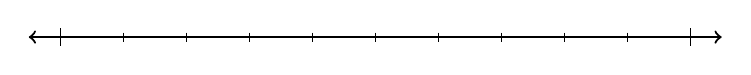
\begin{tikzpicture}[scale=0.8]
% a straight line segment
\draw [thick, <->] (-0.5,0) -- (10.5,0);
% the ticks and their labels
 \draw[xshift=0 cm] (0pt,4pt) -- (0pt,-4pt) ; 
\foreach \x  in {1,...,9}
  \draw[xshift=\x cm] (0pt,2pt) -- (0pt,-2pt);
 \draw[xshift=10 cm] (0pt,4pt) -- (0pt,-4pt) ; 
\end{tikzpicture}

\vspace{1.2cm}

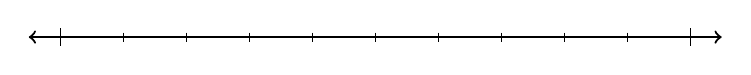
\begin{tikzpicture}[scale=0.8]
% a straight line segment
\draw [thick, <->] (-0.5,0) -- (10.5,0);
% the ticks and their labels
 \draw[xshift=0 cm] (0pt,4pt) -- (0pt,-4pt) ; 
\foreach \x  in {1,...,9}
  \draw[xshift=\x cm] (0pt,2pt) -- (0pt,-2pt);
 \draw[xshift=10 cm] (0pt,4pt) -- (0pt,-4pt) ; 
\end{tikzpicture}

\vspace{0.4cm}

\end{problem}

\begin{problem}
How would your plotted points in the four number lines have been different if the number had been 341.7?  What about 0.003417?  Or 34,170,000?   What does your answer say about the consistent structure of the base-ten place value system?  (Hint:  In each number, how does the meaning of the 4 compare to the meaning of the 1 to its right?   How does the meaning of the 4 compare to the meaning of the 3 to its left?)  

\end{problem}

\begin{problem}
How would your plotted points in the four number lines have been different if the number had been 3.41708?  What about 3.41708667999?  Explain.  

\end{problem}

\begin{problem}
You should know or be able to figure out (in your head) decimal equivalents of fractions with many small  or ``nice'' denominators (i.e., 2, 3, 4, 5, 6, 8, 9, 10, 11, 12, 16, 20, 25, 30, 40, and 50).  Describe how to figure out quickly any that you might forget.  

\end{problem}

\begin{problem}
Here is a nice relationship between twelfths and eighths:  $1/8\approx 0.12$ and $1/12\approx 0.08$.  Find other such pairs, and explain why the pairs ``work'' this way.   

\end{problem}

\begin{problem}
Compare the decimal representations of $\frac{1}{7}$, $\frac{2}{7}$, $\frac{3}{7}$, $\frac{4}{7}$, $\frac{5}{7}$, and  $\frac{6}{7}$.
\begin{enumerate}  
\item Notice that the repeating digits always appear in the same order.  Explain why this is the case.
\item Suppose you are able to remember the decimal representation of $\frac{1}{7}$.  Explain how to use that to write quickly the decimal representation of any of the other sevenths.  
\end{enumerate}
\end{problem}

\begin{problem}
Compare the decimal representations of $\frac{1}{13}$, $\frac{2}{13}$, \dots,  $\frac{12}{13}$.  
\begin{enumerate}  
\item Describe carefully how the order of the digits is somewhat like and also different from what you noticed for sevenths.  
\item Explain why the decimal representations of thirteenths work as you described.
\end{enumerate}
\end{problem}

\begin{problem}
Without a calculator, predict whether the decimal representations of the following numbers will terminate or not.  For those that terminate, predict the number of decimal places.  
\begin{enumerate}
\item $\dfrac{13}{400}$
\item $\dfrac{11}{70}$
\item $\dfrac{21}{70}$
\item $\dfrac{27}{6250}$
\item $\dfrac{23}{2^7\cdot 5^2}$
\item $\dfrac{23}{2^7\cdot 5^2\cdot 11}$
\item $\dfrac{22}{2^7\cdot 5^2\cdot 11}$
\end{enumerate}
\end{problem}

\begin{problem}
The clearest way to demonstrate that a number is rational is to show that it satisfies the definition.  (What is the definition of a rational number?)  Show that the following numbers are rational:  
\begin{enumerate}
\item $0.\overline{324}$
\item $15.\overline{324}$
\item $0.15\overline{324}$
\item $0.2\overline{5643}$
\end{enumerate}
\end{problem}

\subsection*{Generalizations}

\begin{problem}
Use long division to explain why the decimal representation of a rational number must either terminate or repeat.
\end{problem}

\begin{problem}
Suppose $\frac{m}{n}$ is a rational number in lowest terms.  If the number's decimal representation terminates, what can you conclude about $m$ and about $n$?  Explain.  
\end{problem}

\begin{problem}
Suppose $\frac{m}{n}$ is a rational number in lowest terms.  If you know the number's decimal representation repeats, what can you conclude about the number of repeating digits?  Explain.  
\end{problem}

\begin{problem}
You have seen three types of decimal representations for rational numbers between 0 and 1:  terminating, repeating, and delayed-repeating.  Suppose that $m$ and $n$ are counting numbers with no common factors and $m<n$.  Explain why the type of decimal representation of $\frac{m}{n}$ depends only on $n$ and not on $m$.  Hint:  Consider the three types separately.  
\end{problem}

\subsection*{Explorations}

\begin{problem}
The rational number $\frac{1}{19}$ has decimal representation $0.\overline{052631578947368421}$.  To verify this, your calculator is unlikely to display enough digits, and long division would be quite tedious.  Devise a method for ``piecing together'' this decimal representation in ``chunks,'' using your calculator.  Then use the method to compute the decimal representation of $\frac{7}{23}$.  Be sure to indicate how you know that it repeats as you claim.  
\end{problem}

\begin{problem}
Given a prime number $p$, find the smallest positive integer $n$ so that $p$ divides $10^n-1$, or explain why there is no such integer $n$.  
\begin{enumerate}
\item Do this for all primes less than 15, and also for the primes 37, 41, 73, and 101.
\item For each prime, compare the $n$ you found with the number of repeating digits in the decimal representation of $\frac{1}{p}$.  
Make a conjecture about what you notice.  Provide a brief explanation of why your conjecture ought to be true. 
\end{enumerate}
\end{problem}

% In the following two problems, keep in mind that you are trying to explain arithmetic of decimals, which you will teach in grade 5.  
% So your explanations should NOT USE arithmetic of decimals.  Use fractions and the meanings of 
% decimals instead.  And it would be better if you do not use %negative exponents, which is in grade 8.

\begin{problem}
Explain the algorithm for multiplication of decimals in \textbf{two different ways} using $2.7\times 3.4$ as an example.  Be sure your explanations address two key questions:  (i) Why can you almost ignore the decimal point and multiply as though the digits described whole numbers?  And (ii) How do you know where to place the decimal point in the result?  Here are some ideas:  
\begin{itemize}
\item Use behind the scenes algebra to explain why the digits in the  $27\times 34$ should be the same as the digits in the desired product $2.7\times 3.4$.  
\item Convert the decimals to fractions, compute the product of the fractions, and then convert the result to a decimal.  
\item Use the picture below to compute $2.7\times 3.4$ with neither an algorithm nor a calculator.  Explain your reasoning.  
\[
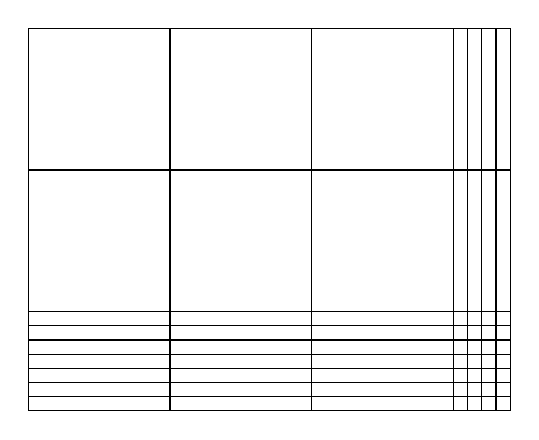
\begin{tikzpicture}[scale=1.8]
%\draw [line width=0.1pt,gray!30,step=1mm] (0,0) grid (3.4,2.7);
%\draw [help lines] (0,0) grid (3.4,2.7);
\draw (0,0) grid (3,2);
\draw [xstep=1cm,ystep=1mm] (0,-0.7) grid (3,0);
\draw [xstep=1mm,ystep=1cm] (3,0) grid (3.4,2);
\draw [xstep=1mm,ystep=1mm] (3,-0.7) grid (3.4,0);
\end{tikzpicture}
\]
\item Explain why the above picture can also represent $27\times 34$.  Explain the lengths and areas for both calculations.  
\end{itemize}
\end{problem}

\begin{problem}
Explain the algorithm for division of decimals in \textbf{two different ways} using $3.96\div 2.4$ as an example.  Be sure your explanations address two key questions:  (i) Why can you almost ignore the decimal point and divide as though the digits described whole numbers?  And (ii) How do you know where to place the decimal point in the result?  Here are some ideas:  
\begin{itemize}
\item Use the measurement model of division to reason how many groups of size $2.4$ are in $3.96$.
\item Use bundles or base ten blocks where the single stick or unit block represents a quantity other than 1.  
\item Multiply both the dividend and the divisor by a suitable power of 10 and then divide.  
\item Convert both decimals to fractions, divide the fractions, then convert the result back to a decimal.  
\item Divide $396$ by $24$ and then use estimation to place the decimal point.  
\end{itemize}
\end{problem}



\end{document}